% !TEX root = ../thesis.tex
%
\chapter{Methodology}
\label{sec:methodology}

% \cleanchapterquote{Innovation distinguishes between a leader and a follower.}{Steve Jobs}{(CEO Apple Inc.)}

\section{Data Collection}
\label{sec:methodology:data}

% \begin{figure}[htb]
% 	
\includegraphics[width=\textwidth]{gfx/Clean-Thesis-Figure}
% 	\caption{Figure example: \textit{(a)} example part one, \textit{(c)} example part two; \textit{(c)} example part three}
% 	\label{fig:system:example1}
% \end{figure}

% \blindtext

% \blindtext

% \begin{figure}[htb]
% 	
\includegraphics[width=\textwidth]{gfx/Clean-Thesis-Figure}
% 	\caption{Another Figure example: \textit{(a)} example part one, \textit{(c)} example part two; \textit{(c)} example part three}
% 	\label{fig:system:example2}
% \end{figure}

% \blindtext
% 3. Methodology
% (1) Purposes; (2) Challenges; (3) Your methodology (including data collection, data analysis, data visualization, etc.); (4) Implementation

\begin{figure}[htb]
	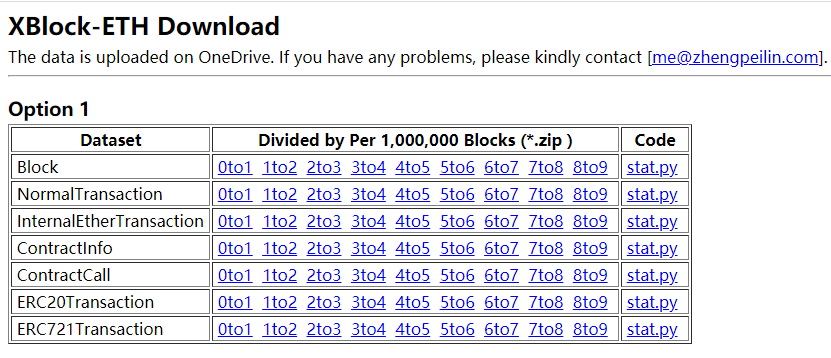
\includegraphics[width=\textwidth]{gfx/data.png}
	\caption{Datasets of Ethereum Transactions}
	\label{fig:data}
\end{figure}

Google BigQuery provides a public dataset which contains updated information of Ethereum transactions. However, it adds complexity in configuring Google account to retrieve data greater than 1 GB, and data size in this thesis is above 100 GB. As an alternative, this thesis adopts data that comes from Xblock website \cite{21}. The datasets of Ethereum transactions are shown in Fig. \ref{fig:data}.

For dataset "Block", it records information related to blocks and its data fields include "blockNumber", "timestamp", "gasUsed", "miner", "reward" and others. For dataset "NormalTransaction", it records information related to external transactions and its data fields include "blockNumber", "timestamp", "from", "to", "creates", "value" and others. For dataset "InternalEtherTransaction", it records information related to internal transactions and its data fields include "blockNumber", "timestamp", "from", "to", "fromIsContract", "toIsContract", "value" and others. For dataset "ContractInfo", it records information related to contract creation and decreation and its data fields include "address", "createdTimestamp", "creator", "decreatedTimestamp", "refunder", "refundValue" and others. When a smart contract is decreated (or deleted), it costs gas to compensate miners for executing this transaction, then some refund value is sent from the refunder to specific accounts. For dataset "ContractCall", it records information related to contract invocation (or call) and its data fields include "blockNumber", "timestamp", "from", "to", "fromIsContract", "toIsContract", "value" and others. When a smart contract is called, it is executed to perform operations defined in contract code. For dataset "ERC20Transaction", it records information related to ERC20 tokens and its data fields include "blockNumber", "timestamp", "tokenAddress", "from", "to", "value" and others. For dataset "ERC721Transaction", it records information related to ERC721 tokens and its data fields include "blockNumber", "timestamp", "tokenAddress", "from", "to", "tokenId" and others. ERC20 and ERC721 are two design standards for Ethereum tokens, they facilitate the development of smart contracts for token issuance and comparison among different tokens. Tokens are frequently used for fundraising and play a similar role as shares of listed companies.

These datasets cover the Ethereum transactions from block 0 on 30 Jul 2015 to block 8,999,999 on 25 Nov 2019. The dataset "ContractInfo" forms the statistical data to compute descriptive statistics and to formulate regression model for investigating the growth of contract activities. Datasets "NormalTransaction", "InternalEtherTransaction", "ContractInfo" and "ContractCall" form the graph data to construct MFG, CCG and CIG for graph visualization of evolving transaction activities.

\subsection{Statistical Data}
\label{sec:methodology:data:statistical}

\begin{figure}[htb]
	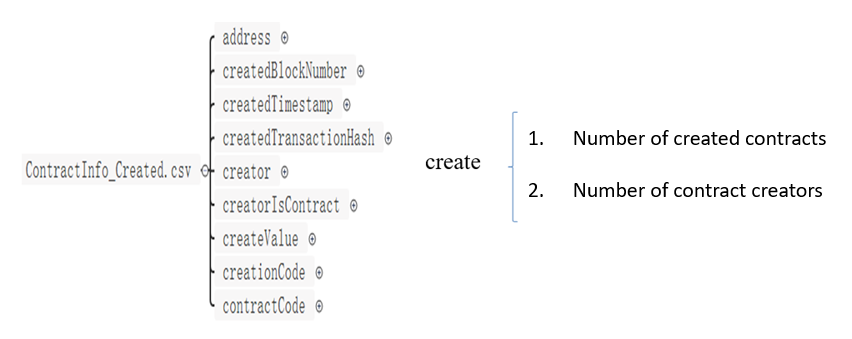
\includegraphics[width=0.95\textwidth]{gfx/statistical1.png}
	\caption{Data fields for contract creation}
	\label{fig:statistical1}
\end{figure}

\begin{figure}[htb]
	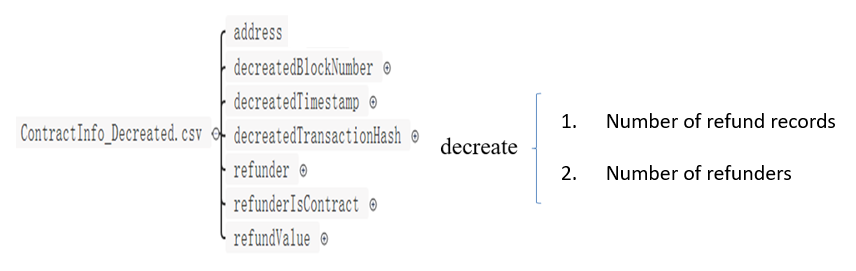
\includegraphics[width=\textwidth]{gfx/statistical2.png}
	\caption{Data fields for contract decreation}
	\label{fig:statistical2}
\end{figure}

The dataset "ContractInfo" consists of transaction information related to smart contract creation and decreation.

Transactions for smart contract creation are recorded with data fields shown in Fig. \ref{fig:statistical1}, these transactions are grouped by day to compute the metrics including daily number of created contracts and daily number of contract creators. Then, the metrics are used to compute descriptive statistics and to draw time plots.

Transactions for smart contract decreation are recorded with data fields shown in Fig. \ref{fig:statistical2}, these transactions are grouped by day to compute the metrics including daily number of refund records and daily number of refunders. Then, the metrics are used to compute descriptive statistics and to draw time plots. They are also used to formulate a regression model that describes the correlated factors of refund.

\subsection{Graph Data}
\label{sec:methodology:data:graph}

The relevant datasets are processed in the following order:

1. The dataset "ContractInfo" is used to obtain all "ccg\_nodes" and "ccg\_edges" of CCG data. For "ccg\_nodes", its "node\_name" and "node\_type" are determined by "address" in "ContractInfo". For "ccg\_edges", its "from\_name", "to\_name", "time\_stamp" are determined by "creator", "address", "createdTimestamp" in "ContractInfo".

2. The dataset "ContractCall" is used to obtain all "cig\_nodes" and "cig\_edges" of CIG data. For "cig\_nodes", its "node\_name" and "node\_type" are determined by "from", "fromIsContract", "to", "toIsContract" in "ContractCall". For "cig\_edges", its "from\_name", "to\_name", "time\_stamp", "number\_of\_calls" are determined by "from", "to", "timestamp" in "ContractCall".

3. The dataset "InternalEtherTransaction" is used to obtain partial "mfg\_nodes" and "mfg\_edges" of MFG data. For "mfg\_nodes", its "node\_name" and "node\_type" are determined by "from", "fromIsContract", "to", "toIsContract" in "InternalEtherTransaction". For "mfg\_edges", its "from\_name", "to\_name", "time\_stamp", "value\_in\_ether" are determined by "from", "to", "timestamp", "value" in "InternalEtherTransaction".

4. The dataset "NormalTransaction" is used to obtain remaining "mfg\_nodes" and "mfg\_edges" of MFG data. For "mfg\_nodes", its "node\_name" and "node\_type" are determined by "from", "fromIsContract", "to", "toIsContract" in "NormalTransaction". For "mfg\_edges", its "from\_name", "to\_name", "time\_stamp", "value\_in\_ether" are determined by "from", "to", "timestamp", "value" in "NormalTransaction".

During the extraction of graph data, the addresses of exchanges are converted to their names for identification of exchanges later in graph visualization, the address-name pairs of exchanges are found in exchange directory on EtherScan \cite{17}. Finally, the extracted nodes and edges are stored as collections in a database called "ethereum\_tx".

\section{Statistical Analysis}
\label{sec:methodology:analysis}

\subsection{Descriptive Statistics}
\label{sec:methodology:analysis:statistics}

\begin{table}[h]
\caption{Example of descriptive statistics}
\label{tab:descriptive-statistics}
\renewcommand\arraystretch{0.7}
\begin{tabular}{@{}cc@{}}
\toprule
\multicolumn{2}{c}{Daily number of created contracts} \\
\midrule
Average                & 12267.14442    \\
Standard Error         & 366.8075104    \\
Median                 & 7510.5         \\
Mode                   & 7267           \\
Standard Deviation     & 11089.48345    \\
Variance               & 122976643.2    \\
Kurtosis               & 2.305335977    \\
Skewness               & 1.789698857    \\
Minimum                & 650            \\
Maximum                & 52959          \\
Summation              & 11212170       \\
Observation            & 914            \\
\bottomrule
\end{tabular}
\end{table}

\begin{figure}[htb]
	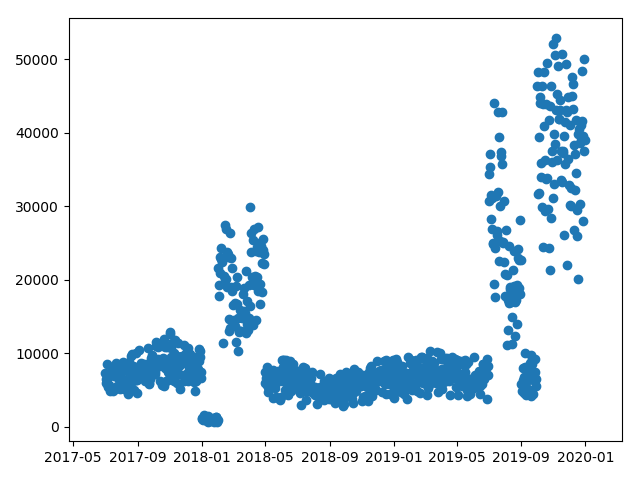
\includegraphics[width=0.7\textwidth]{gfx/created-contracts.png}
	\caption{Example of a time plot}
	\label{fig:created-contracts}
\end{figure}

Statistical data representing contract creation and contract decreation is used to compute descriptive statistics and to draw time plots. An example of descriptive statistics is shown in Table \ref{tab:descriptive-statistics}, these statistics describe the distribution of metric for all observation days with "Average", "Standard Error", "Median", "Mode, "Standard Deviation", "Variance", "Kurtosis", "Skewness", "Minimum", "Maximum", "Summation" and "Observation". Moreover, the change of metric is illustrated by a time plot to visualize its trend, an example is shown in Fig. \ref{fig:created-contracts}.

\subsection{Regression Model}
\label{sec:methodology:analysis:model}

\begin{table}[h]
\caption{Correlation coefficient matrix}
\label{tab:correlation-matrix}
\begin{tabular}{|c|c|c|c|c|c|c|}
\hline
\multicolumn{7}{|c|}{Correlation coefficient matrix} \\
\hline

\multicolumn{2}{|c|}{} &
\makecell{Created\\ Contracts} & \makecell{Contract\\ Creators} & \makecell{Refund\\ Records} & Refunders & \makecell{Refund\\ Amount} \\
\hline

\multirow{2}{*}{
\makecell{Created\\ Contracts}} & Related & 1 & -0.038 & .169** & .253** & -.148** \\
\cline{2-7} & significant & & 0.256 & 0.000 & 0.000 & 0.000 \\
\hline
\multirow{2}{*}{Contract Creators} & Related & -0.038 & 1 & .349** & .153** & -0.017 \\
\cline{2-7} & significant & 0.256 & & 0.000 & 0.000 & 0.605 \\
\hline
\multirow{2}{*}{
\makecell{Refund\\ Records}} & Related & .169** & .349** & 1 & .426** & -0.005 \\
\cline{2-7} & significant & 0.000 & 0.000 & & 0.000 & 0.878 \\
\hline
\multirow{2}{*}{Refunders} & Related & .253** & .153** & .426** & 1 & -.148** \\ 
\cline{2-7} & significant & 0.000 & 0.000 & 0.000 & & 0.000 \\
\hline
\multirow{2}{*}{
\makecell{Refund\\ Amount}} & Related & -.148** & -0.017 & -0.005 & -.148** & 1 \\
\cline{2-7} & significant & 0.000 & 0.605 & 0.878 & 0.000 &  \\[10pt]
\hline
\multicolumn{7}{|l|}{*. At level 0.05, the correlation was significant} \\ 
\hline
\multicolumn{7}{|l|}{**. At level 0.01, the correlation was significant} \\ 
\hline
\end{tabular}
\end{table}

Regarding the daily refund amount, the potentially correlated variables including daily number of created contracts as "Created Contracts", daily number of contract creators as "Contract Creators", daily number of refund records as "Refund Records", daily number of refunders as "Refunders", daily refund amount as "Refund Amount" are investigated with the correlation coefficient matrix in Table \ref{tab:correlation-matrix}. The correlation coefficients in the matrix are Pearson correlation coefficients. In Table \ref{tab:correlation-matrix}, the rows "Related" and "significance" contain the test statistics of correlation coefficients for each pair of variables and their significance under two-tailed hypothesis testing respectively. If the significance is below a level, 0.05 or 0.01, it is said to be statistically significant to conclude that the pair of variables are correlated.

From the results of correlation coefficient matrix, the daily refund amount is statistically correlated to the daily number of created contracts and daily number of refunders both at significance level 0.01. Therefore, the daily number of created contracts and daily number of refunders are fitted to linear regression model to predict the daily refund amount. The regression statistics are shown in Table \ref{tab:regression-statistics}.

\begin{table}[h]
\caption{Regression Statistics}
\label{tab:regression-statistics}
\begin{tabular}{c|c}
\hline
\multicolumn{2}{c}{Regression Statistics} \\
\hline
Multiple R & .839a \\
\hline
R Square & .704 \\
\hline
Adjusted R Square & .653 \\
\hline
Standard Error & 320.299643300000000 \\
\hline
Observations & 914 \\
\hline
\end{tabular}\\
\end{table}

From the regression statistics, the R Square is 70.4\%, it means that 70.4\% of variation in daily refund amount can be explained by the daily number of created contracts and daily number of refunders. In addition, the Analysis Of Variance (ANOVA) is performed to further investigate the relations between these variables, the results are provided in Table \ref{tab:anova-table}.

\begin{table}[h]
\caption{ANOVA Table}
\label{tab:anova-table}
\begin{tabular}{c|c|c|c|c}
\hline
\multicolumn{5}{c}{ANOVA Table} \\
\hline
 & Coefficients & Standard Error & t Stat & P-value \\
\hline
Intercept & 183.198 & 25.191 & 7.273 & .000 \\
\hline
Created Contracts & -0.005 & .001 & -4.953 & .000 \\
\hline
Refunders & .081 & .026 & 3.102 & .002 \\
\hline
\end{tabular}
\end{table}

From ANOVA table, the P-values of intercept, daily number of created contracts and daily number of refunders are all below 0.01, it implies they are statistically significant to be included in the linear regression model. By considering the coefficients of these explanatory variables, the resultant regression model can be written as:

$$\text{Refund Amount} = 183.198 - 0.005 * \text{Created Contracts} + 0.081 * \text{Refunders}$$

\section{Graph Visualization}
\label{sec:methodology:view}

\begin{table}[h]
\caption{Development Challenges}
\label{tab:development-challenges}
\begin{tabular}{@{}cc@{}}
\toprule
Challenge & Module      \\
\midrule
Interactive UI & PyQt5       \\
Large graph visualization & Vispy       \\
Large graph layout & PyGraphviz  \\
Portable program & PyInstaller \\
\bottomrule
\end{tabular}
\end{table}

The major development challenges for graph visualization of Ethereum transactions are listed in Table \ref{tab:development-challenges}, they include interactive User Interface (UI), large graph visualization, large graph layout, portable executable program. These challenges are handled by the following Python modules.

PyQt5 represents UI elements as Python classes, their style can be modified by changing the property values while their behavior can be altered by linking to a function \cite{2}. The built-in Qt designer can be used to create UI elements and convert them into code, then only the functions need to be programmed.

Vispy leverages the computing power of GPU to achieve high performance in large data visualization \cite{12}. It is mainly applied to filtering out the subgraph and computing the graph analytics (i.e. centrality and community measures).

PyGraphviz provides fast algorithms of generating large graph layout which avoids overlapping edges for clear visualization \cite{15}.

PyInstaller is a light-weight packaging manager to convert Python program to executable, in this paper it is used to create portable version of the program \cite{20}.

The program for graph visualization is shown in Fig. \ref{fig:view}. It is composed of four core components, namely data view (Fig. \ref{fig:view}A), graph view (Fig. \ref{fig:view}B), node view (Fig. \ref{fig:view}C) and control view (Fig. \ref{fig:view}D).

\begin{figure}[htb]
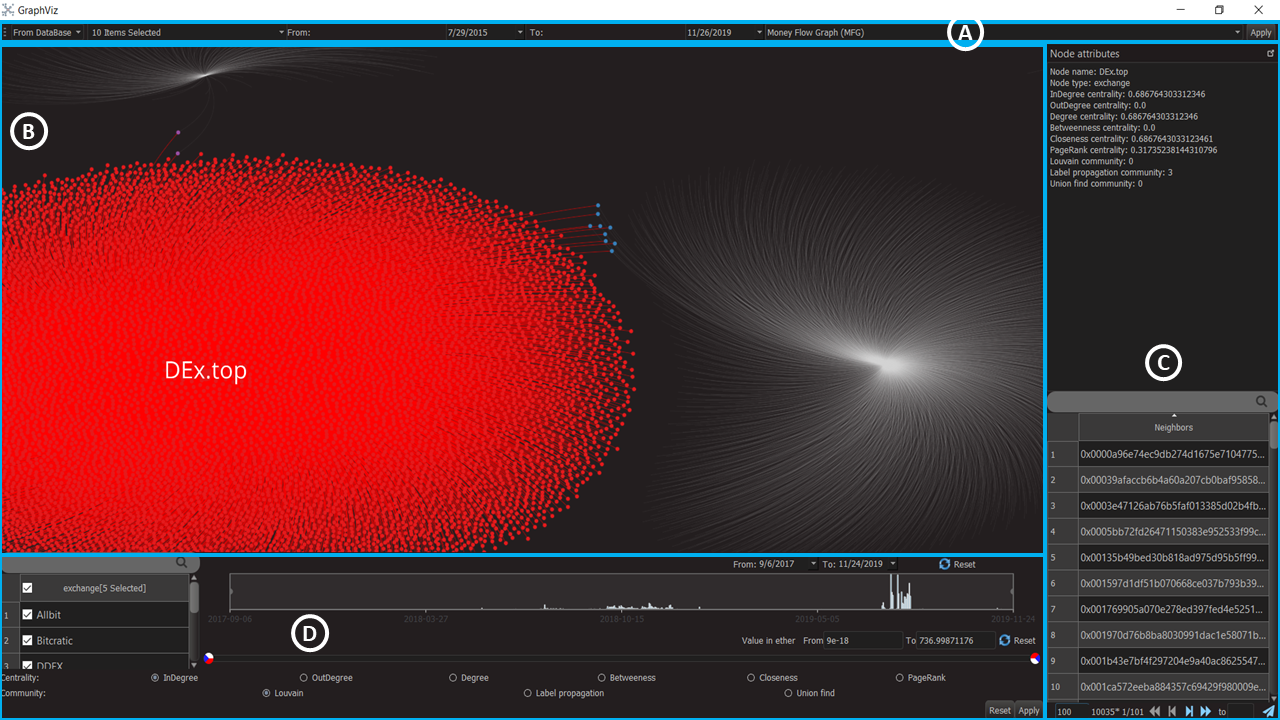
\includegraphics[width=\textwidth]{gfx/view.png}
\caption{Graph visualization is divided into four components including (A) data view, (B) graph view, (C) node view and (D) control view.}
\label{fig:view}
\end{figure}

\subsection{Data View}
\label{sec:methodology:view:data}

\begin{figure}[htb]
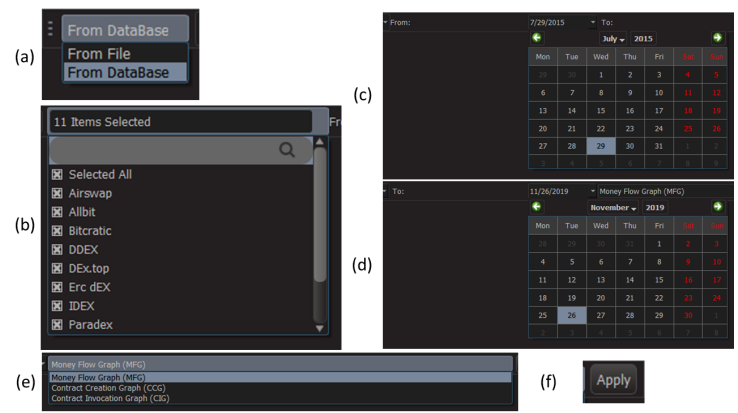
\includegraphics[width=0.7\textwidth]{gfx/data-view.png}
\caption{Data view consists of (a) options to select data source, (b) options to select exchange names, (c) options to select starting date, (d) options to select ending date, (e) options to select graph type and (f) retrieval of data under selection criteria.}
\label{fig:data-view}
\end{figure}

The data view acts as a menu bar for users to specify the selection criteria to retrieve data from the data source. The available options are in the groups of data source (Fig. \ref{fig:data-view}a), exchange names (Fig. \ref{fig:data-view}b), starting date (Fig. \ref{fig:data-view}c), ending date (Fig. \ref{fig:data-view}d) and graph type (Fig. \ref{fig:data-view}e). The "Apply" button (Fig. \ref{fig:data-view}f) combines these selection options to retrieve data for graph construction.

The selection of data source is to retrieve transactions from either a GEXF file or the MongoDB database. GEXF format is the default format in Gephi representing data structure of graph in the form of nodes and edges.

The selection of exchange names is to retrieve transactions where each transaction has its from address or to address in the list of selected exchanges. The exchange names are grouped by exchange type and sorted alphabetically.

The selection of starting date and ending date is to retrieve transactions occurred between these two dates. The default starting date is one day before the first transaction while the default ending date is one day after the last collected transaction.

The selection of graph types is to retrieve transactions based on three major activities, namely MFG for money transfer, CCG for contract creation, CIG for contract invocation.

Moreover, the program supports the opening of multiple windows which facilitates the comparison analysis. For examples, transactions for the same exchanges in different time periods can be compared in different windows, or transactions for different categories such as crypto exchanges and decentralized exchanges can be compared in different windows.

\subsection{Graph View}
\label{sec:methodology:view:graph}

\begin{figure}[htb]
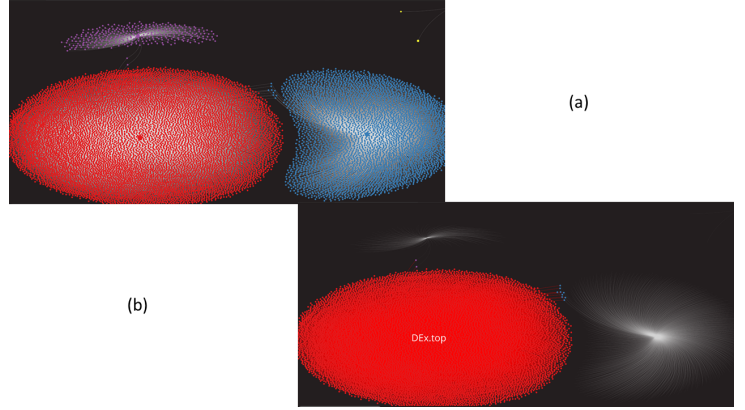
\includegraphics[width=0.7\textwidth]{gfx/graph-view.png}
\caption{Graph view shows the effects of nodes and edges (a) before clicking a node and (b) after clicking a node.}
\label{fig:graph-view}
\end{figure}

The graph view is used to display the nodes and edges after graph construction. Before clicking a node (Fig. \ref{fig:graph-view}a), nodes of different sizes and colors are connected by light gray edges. After clicking a node (Fig. \ref{fig:graph-view}b), the clicked node and all its neighbor nodes are highlighted while the other nodes become transparent. Besides, the name of clicked node is popped up.

\subsection{Node View}
\label{sec:methodology:view:node}

\begin{figure}[htb]
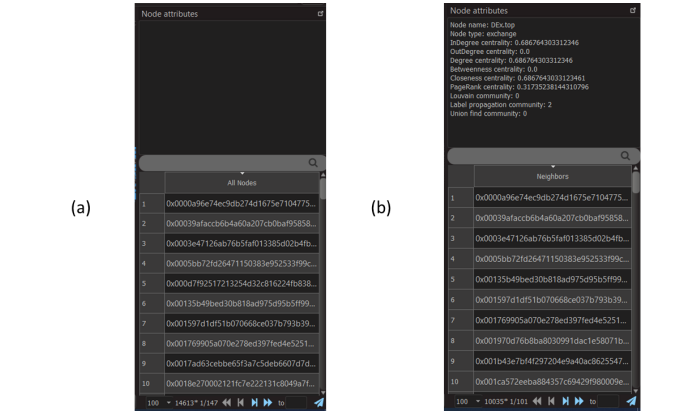
\includegraphics[width=\textwidth]{gfx/node-view.png}
\caption{Node view displays attribute values and names of nodes (a) before clicking a node and (b) after clicking a node.}
\label{fig:node-view}
\end{figure}

The node view is to list out the information of a clicked node. Before clicking a node (Fig. \ref{fig:node-view}a), the values of node attributes are blank, and a list of all nodes is shown below the node attributes. After clicking a node (Fig. \ref{fig:node-view}b), the values of node attributes are displayed, and its neighbor nodes are shown below the node attributes.

\subsection{Control View}
\label{sec:methodology:view:control}

\begin{figure}[htb]
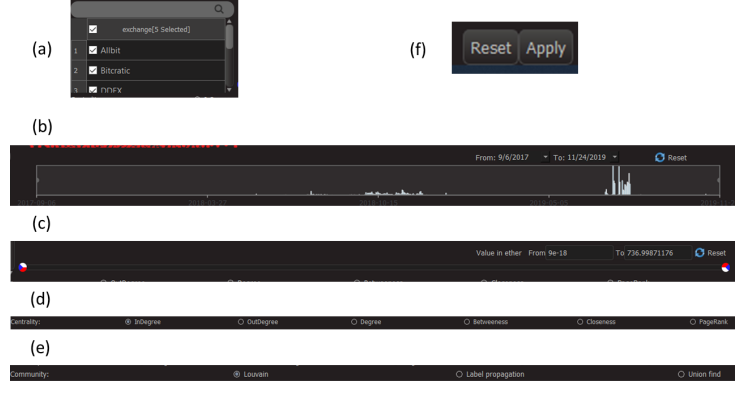
\includegraphics[width=\textwidth]{gfx/control-view.png}
\caption{Control view includes (a) options to filter the selected exchanges, (b) time brush to filter transactions within a specific period, (c) value slider to filter transactions within a specified range, (d) options to select a centrality measure, (e) options to select a community measure, and (f) "Reset" and "Apply" buttons.}
\label{fig:control-view}
\end{figure}

The control view contains filters of transactions for selected exchanges (Fig. \ref{fig:control-view}a), selected time interval (Fig. \ref{fig:control-view}b), and corresponding value range (Fig. \ref{fig:control-view}c), and selection options of centrality measure (Fig. \ref{fig:control-view}d) and community measure (Fig. \ref{fig:control-view}e). The "Reset" button sets the filters and selections to default values while the "Apply" button sets the filters and selections effective.

After filtering the transactions by exchange, a subgraph contains only those nodes and edges to represent the transactions with from address or to address as the specified exchanges.

After filtering the transactions by a time brush, a subgraph containing nodes and edges to represent transactions within the specified time interval is present. To observe the evolution of graph structure or the changes of graph over time, the time brush starts from a fixed time point, then it is moved at increments with the "Apply" button being pressed. As a result, the "growth" of graph can be revealed for evolution analysis.

After filtering the transactions by a value slider, the transactions within the specified value range are represented by a subgraph of nodes and edges, this value range refers to value in ether for MFG and number of calls for CIG and is not applicable for CCG. To observe the transactions at increasing weight, the value slider has a fixed end, then it is moved to right gradually with the "Apply" button taking effect. As a result, the graph with high edge weights "floats" on the surface.

The selection options for centrality measures consist of in-degree centrality, out-degree centrality, degree centrality, betweenness centrality, closeness centrality and PageRank centrality. The centrality value is positively correlated to the node size.

The selection options for community measures include Louvain community, label propagation community and union find community. The community cluster which a node is assigned to determines the node color.

% \section{Conclusion}
% \label{sec:system:conclusion}

% \blindtext
